\section{Results and Discussions}
\label{chap:results}

The results presented in this chapter are corrected for acceptance effects, 
but not for radiative ones. We use the following DIS selection cuts: 
$Q^2$~$>$~$1$~GeV$^2$/c$^2$, $W$~$>$~$2$ GeV and $y<0.85$. In order to ensure that 
factorization applies, we select $0.4$~$<$~$z$~$<$~$0.7$\footnote{This cut is not 
applied for plots as a function of $z$.}, this choice is based on experimental results from 
\cite{Asaturyan:2011mq}. Moreover, this cut also ensures that we measure the leading 
hadron and that we avoid the high $z$ region, which might be contaminated by 
the diffractive $\rho^0$ decay products. Finally, the cut $x_F > 0$ select the 
current fragmentation region.

\subsection{Multiplicity Ratio}

\subsubsection{$A$ Dependence}
\label{sec:resA}

\begin{figure}[p]
\centering
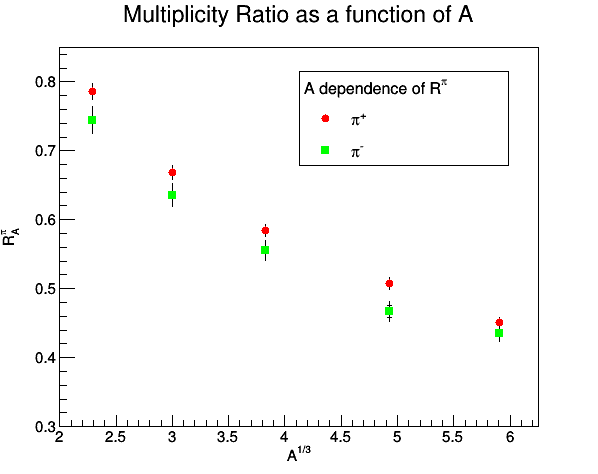
\includegraphics[width=7.4cm] {chap6-fig/F_RvA.png} 
\caption {$A^{1/3}$ dependence of the multiplicity ratio. Normalization 
uncertainties are not shown.}
\label{fig:RA}
\end{figure}

The figure \ref{fig:RA} presents our result for the $A^{1/3}$ dependence of 
the multiplicity ratio. One can see a 5\% normalization difference between
pions. However, this difference is not significant as it represents only 1.5 
standard deviation of our normalization uncertainty (see table~\ref{tab:sysid}).

The attenuation, presented in the figure \ref{fig:RA}, is not linear as 
a function of $A^{1/3}$ nor $A^{2/3}$. HERMES data has already showed some indication 
of this feature \cite{Airapetian:2007vu,Airapetian:2009jy}, but here, the nonlinearity, 
which has important implication on models, is clear. Indeed, it seems difficult 
to conciliate the prehadron absorption models with this result. Prehadrons 
are expected to have their cross section increasing with time and, therefore, 
distance. On the parton energy loss side, the BDMPS calculation gives a parton energy loss proportional to 
$L^2 \propto A^{2/3}$ also in contradiction with this result. However, 
this statement does not hold at low energy and might also be 
modified if the production time occurs inside the nuclei.

\subsubsection{Cronin Effect}

\begin{figure}[p]
\centering
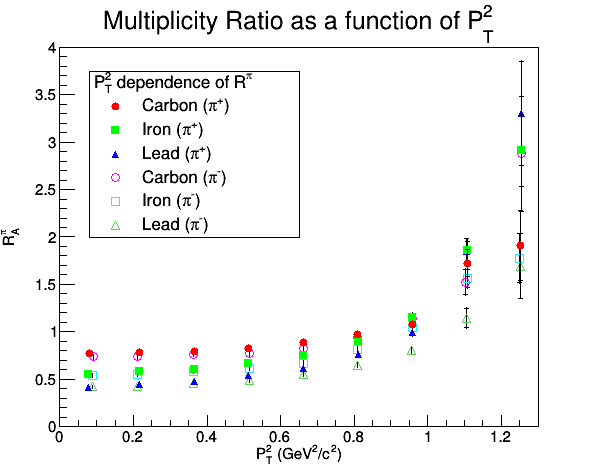
\includegraphics[width=7.4cm] {chap6-fig/F_RvPt.png} 
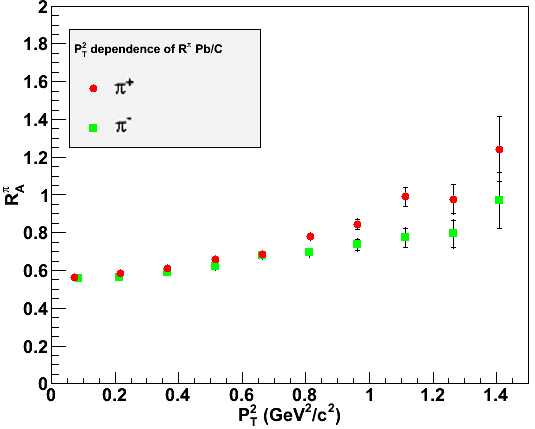
\includegraphics[width=7.4cm] {chap6-fig/F_RvPt_PbC.png} 
\caption {Multiplicity ratios as a function of \pt (GeV$^2$/c$^2$) for charged pions. Left panel is 
the usual observable, right panel shows multiplicity ratio of lead normalized to carbon.
Normalization uncertainties are not shown.}
\label{fig:RPt}
\end{figure}

\begin{figure}[p]
\centering
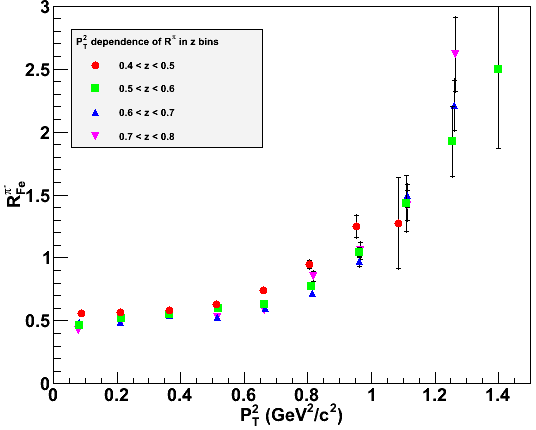
\includegraphics[width=7.4cm] {chap6-fig/F_RvPtinZ.png} 
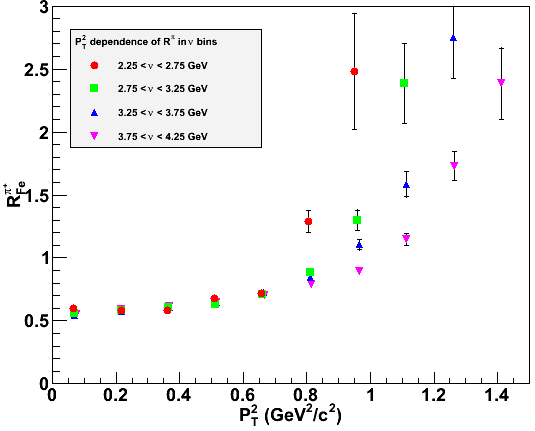
\includegraphics[width=7.4cm] {chap6-fig/F_RvPtinNu.png} 
\caption {Multiplicity ratios as a function of \pt (GeV$^2$/c$^2$) and $z$ (left) 
or $\nu$ (GeV) (right) for positive pions. Normalization uncertainties are not shown.}
\label{fig:RPtMulti}
\end{figure}

The Cronin effect is characterized by a large increase of the multiplicity 
ratio at high \pt ($\sim$1~GeV$^2$/c$^2$), but it is a controversial 
measurement in hadronization studies. Indeed, whereas SLAC measurements 
\cite{Osborne:1978ai} did not show such an effect, HERMES 
\cite{Airapetian:2007vu} measured a significant increase of the multiplicity 
ratio with \ptp. Our result (figure \ref{fig:RPt} (left)), integrated over 
all other variables, shows a pattern similar to the HERMES measurement. 
However, there is potential contributions from the target fragmentation (see 
chapter~\ref{chap:data}) and the Fermi motion (see chapter \ref{chap:pyqm}).

Fermi motion effects can be significantly reduced by modifying 
our usual observables. Indeed, using carbon for normalization, instead of deuterium, 
cancels most of the effects of Fermi motion. Moreover, acceptance 
effects (section~\ref{sec:accept}) are mostly canceled as well in such a ratio, 
reducing various systematic errors (including most of the normalization error). 
The figure \ref{fig:RPt} (right) represents the multiplicity ratio based on carbon. We 
observe an attenuation, at low \ptp, similar to the usual multiplicity ratio 
of iron. This can be understood from the radius of the nuclei $R_{Pb}-R_{C} 
\sim R_{Fe}$. Nevertheless, the observed enhancement with \pt is much more modest than in 
iron. At first sight the difference can be attributed to Fermi motion, which 
might affect the measurement based on deuterium. The target fragmentation 
effects might also lead to similar observation and more evidence are 
needed to confirm our interpretation.

In the figure \ref{fig:RPtMulti}, the multi-dimensionally binned multiplicity 
ratio are presented. HERMES found an important dependence of the Cronin effect 
with $z$ \cite{Airapetian:2007vu,Airapetian:2011jp} that we interpreted as a 
sign of an important target fragmentation contribution. The present result 
(figure~\ref{fig:RPtMulti} (left)) does not show this behavior, but it can be 
explained by our stricter cut on $z$ ($z>0.4$ whereas HERMES uses $z>0.2$), which 
leads to a smaller target fragmentation contamination. The second result, 
binned in \pt and $\nu$ (figure \ref{fig:RPtMulti} (right)), shows an important 
dependence of the Cronin effect with $\nu$. However, HERMES results did not 
reveal any similar $\nu$ variation. This is an evidence of the importance of 
the Fermi motion effect in our measurement. Indeed, in the 
chapter~\ref{chap:pyqm}, it was shown that the impact of Fermi motion gets 
smaller at higher energy.

The result for the lead to carbon multiplicity ratio, figure \ref{fig:RPt} 
(right), has another interesting feature: the $\pi^+$s have a stronger Cronin 
effect. However, the signification of this observation is not clear. This could be 
a contribution from target fragmentation, as we might expect more positive 
particles than negative ones coming from the nuclei.
This could also come from other sources such as isospin effect or factorization breaking at high 
\ptp, but no test of these features exists in this kinematical range\footnote{
\cite{Asaturyan:2011mq} covers only \pt$<0.2$ GeV$^2$/c$^2$.}. Last, it could 
be linked to the hadron rank and reflect some hadronization properties. Indeed, 
as we probe mostly valence quark at our energies, $\pi^+$s are more likely to 
be leading hadron compared to $\pi^-$s.

In conclusion, our results indicate that the HERMES results were affected by target 
fragmentation and that our results are affected by Fermi motion. These effects can 
be easily controlled by selecting carefully our observables and kinematic coverage.

\subsubsection{$\nu$ Dependence}

\begin{figure}[tbp]
\centering
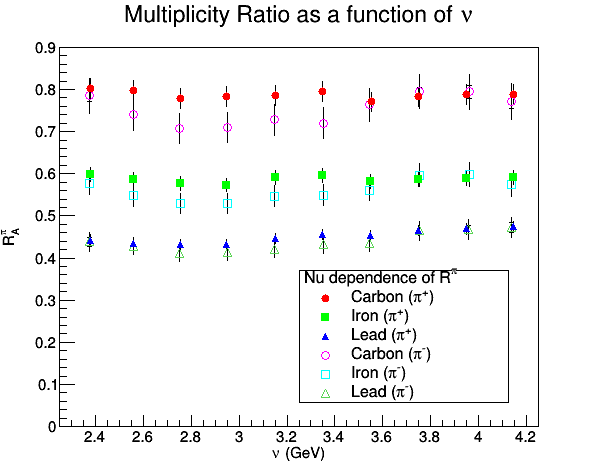
\includegraphics[width=7.4cm] {chap6-fig/F_RvNu.png} 
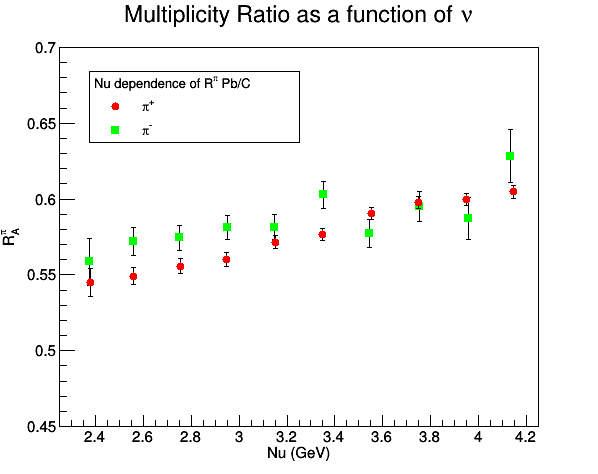
\includegraphics[width=7.4cm] {chap6-fig/F_RvNu_PbC.png} 
\caption{Multiplicity ratios as a function of $\nu$ (GeV). Left panel is the usual 
observable, right panel shows multiplicity ratio of lead normalized to carbon. 
Normalization uncertainties are not shown.}
\label{fig:RNu}
\end{figure}

The HERMES collaboration clearly observed a rise of the multiplicity ratio 
between $\nu$ of 4 and 22~GeV. However, at first sight, in our results (figure 
\ref{fig:RNu} (left)), no dependence is observed, except for a 
slight increase in lead. The results on Fermi motion together 
with the figure \ref{fig:RNu} (right) permit to reach a coherent explanation. The 
Fermi motion seems to cancel the hadronization effect almost completely and the
systematic uncertainties linked with acceptance might wash out what remains of the effect. The 
multiplicity ratio based on carbon, however, offers a very neat slope consistent 
with what was observed on a much larger range by HERMES.

We also notice here that both pions give similar results in the figure 
\ref{fig:RNu} (right). This confirms our previous remark that the difference 
observed in the multiplicity ratio based on deuterium might come from the 
normalization uncertainty caused by the acceptance correction. Therefore, there is no 
clear difference between the charged pions for the integrated multiplicity 
ratios.

\subsubsection{$z$ Dependence}

\begin{figure}[tbp]
\centering
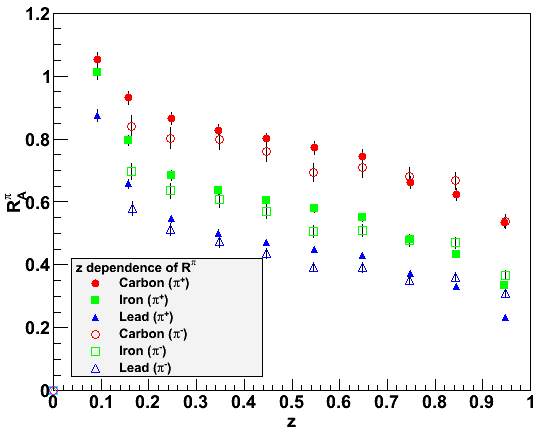
\includegraphics[width=7.4cm] {chap6-fig/F_RvZ.png} 
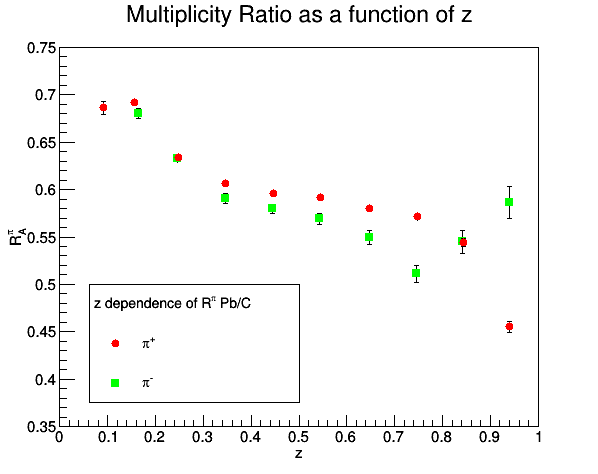
\includegraphics[width=7.4cm] {chap6-fig/F_RvZ_PbC.png} 
\caption {Multiplicity ratios as a function of $z$. Left panel is the usual
observable, right panel shows multiplicity ratio of lead normalized to carbon. 
Normalization uncertainties are not shown.}
\label{fig:Rz}
\end{figure}

The multiplicity ratio was observed to decrease with $z$ in HERMES data, 
whereas this feature was not as significant in other experiments. Indeed the 
nature of this behavior is questionable, the target fragmentation also reduce 
with $z$ and can mimic the effect. In figure \ref{fig:Rz} (left), as in 
HERMES, we see a clear slope even at values higher than 0.4, where target fragmentation
effects are expected to be small. However, the ratio lead to carbon (figure 
\ref{fig:Rz} (right)) shows a much flatter behavior in the region of interest 
(0.4 to 0.7). This is coherent with what we showed in chapter \ref{chap:pyqm}, i.e. the expected $z$ slope 
is enhanced by Fermi motion effects. Therefore, the situation seems to be 
similar to the Cronin effect one, where HERMES observation was enhanced by 
target fragmentation. The measurement using the carbon as basis is, therefore, 
more useful to isolate effects from the hadronization, but low $z$ behavior 
remains driven by the target region. Another strange feature of the data is 
the behavior at high $z$ (figure \ref{fig:Rz} (right)), where the two pions 
behave differently. However, we lack of solid theoretical grounds in this 
region to interpret this result.

\subsubsection{$Q^2$ Dependence}

The behavior of hadronization as a function of $Q^2$ is an important issue, that 
has direct implications on our understanding of nuclear matter properties in 
QCD. HERMES results, which covers $1<Q^2<10$~GeV$^2$/c$^2$, give a hint for an 
increase of the multiplicity ratio with $Q^2$. Our result, in figure 
\ref{fig:RQ2}, does not allow to reach the same conclusion and indicates no 
significant dependence as a function of $Q^2$.

\begin{figure}[tbp]
\centering
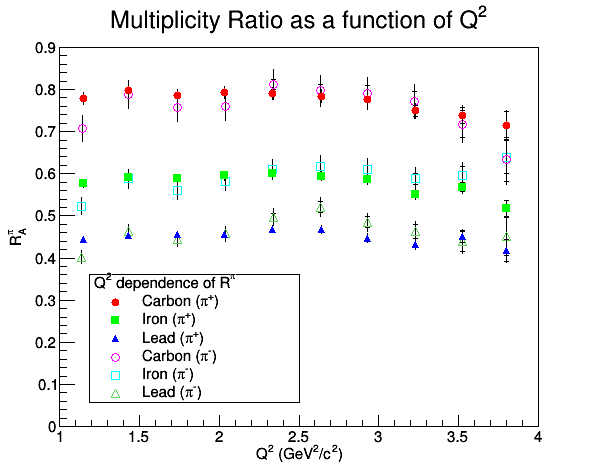
\includegraphics[width=7.4cm] {chap6-fig/F_RvQ2.png} 
\caption {Multiplicity ratios as a function of $Q^2$ (GeV$^2$/c$^2$). 
Normalization uncertainties are not shown.}
\label{fig:RQ2}
\end{figure}

We can use our large statistics to get more information. As 
a dependence in $\nu$ is expected for the multiplicity ratio, it might be helpful to use a tight 
$\nu$ bin to plot the $Q^2$ dependence (figure \ref{fig:RQ2Detailed} (left)), 
and remove any coupling between the two variables.
We could also expect some effects from the Fermi motion, 
therefore, we show in figure \ref{fig:RQ2Detailed} (right) the multiplicity ratio of lead to 
carbon as a function of $Q^2$. The two results of figure \ref{fig:RQ2Detailed} 
show a slight increase with $Q^2$, but as for HERMES, no evidence is 
reached on this question. Our leverage on $Q^2$ appears to be too modest
to make a clear measurement. Future programs to explore this question are 
discussed in chapter~\ref{chap:future}.

\begin{figure}[tbp]
\centering
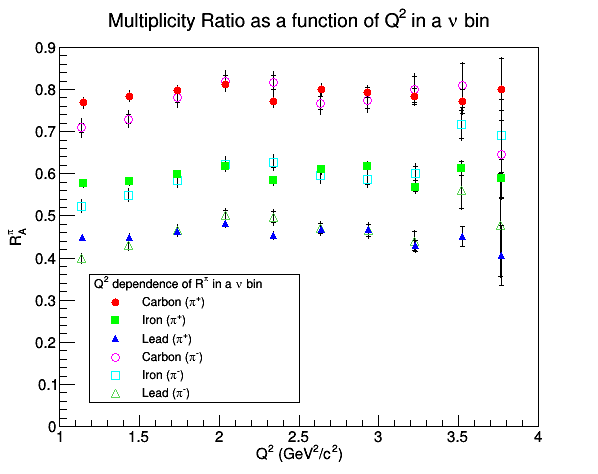
\includegraphics[width=7.4cm] {chap6-fig/F_RvQ2inNu.png} 
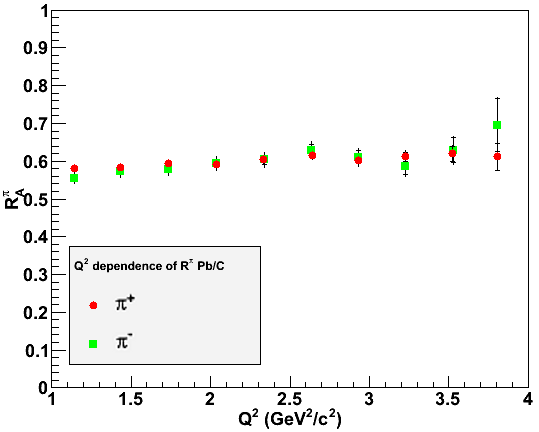
\includegraphics[width=7.4cm] {chap6-fig/F_RvQ2_PbC.png} 
\caption {Multiplicity ratios as a function of $Q^2$ (GeV$^2$/c$^2$). In the left panel,
the multiplicity ratio in a tight $\nu$ bin ($3.25 < \nu < 3.75$ GeV). In the right 
panel, the multiplicity ratio of lead normalized to carbon. Normalization 
uncertainties are not shown.}
\label{fig:RQ2Detailed}
\end{figure}

\subsection{Transverse Momentum Broadening}

\subsubsection{$A$ Dependence}

The $A$ dependence of the transverse momentum broadening, presented in 
figure~\ref{fig:PA}, is an important result. The large statistics coupled with the 
large coverage in $A$ available to the CLAS experiment give precise indication on \dpt 
as a function of $A^{1/3}$. Compared to HERMES \cite{Airapetian:2009jy}, we
find smaller \dptp. This is coherent with theory, which predicts larger effects
at larger energies. However, calculations of parton energy loss from BDMPS 
\cite{Baier:1996sk} show that \pt should depend on the nucleus radii
(see chapter \ref{chap:theory}). However, this feature does not appear in our 
result. Of course, because of the low energy of the CLAS experiment, one might 
discuss the possibility to make a direct comparison with BDMPS calculations. Nonetheless, 
this result shows an unexpected pattern that remains to be explained. One 
possibility is that, as proposed for the multiplicity ratio as a function of 
$A^{1/3}$, the production time occurs inside the nuclei. In this case, the 
colored parton would not interact with the whole nuclei and therefore changing 
its size would lead to limited effect.

\begin{figure}[tbp]
\centering
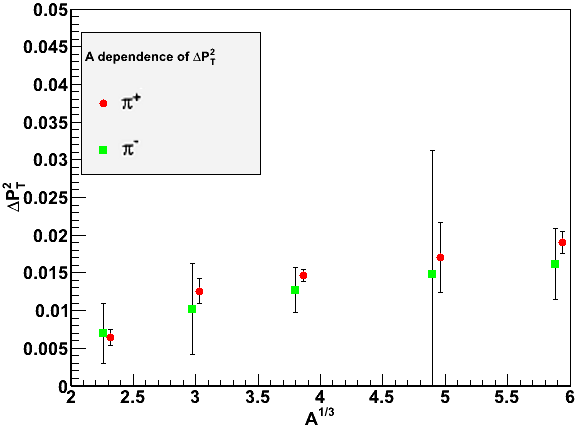
\includegraphics[width=8.2cm] {chap6-fig/F_PvA.png} 
\caption {$A$ dependence of \dptp. Points are slightly offset for readability, normalization uncertainties are not shown.}
\label{fig:PA}
\end{figure}

\subsubsection{$z$ Dependence}

The $z$ dependence of \dpt has some importance for parton energy loss
models, because it is linked to the assumptions needed to extrapolate the hadronic \pt
to the partonic one. Moreover, usually, in parton energy loss models, \dpt
goes to zero at the highest $z$. Our results (figure \ref{fig:PZ}) do
not show such a pattern. However, our previous results showed the importance of 
Fermi motion in our kinematics, which is expected to enhance \dpt at very high
$z$. This is confirmed by the flattening observed for the carbon based \dptp, but
the distribution is not clearly going down either at high $z$. This might be due to the size of the 
error bars and the potential contamination from diffractive $\rho^0$ production, both 
preventing us from any definitive statement on this feature of the data.

\begin{figure}[tbp]
\centering
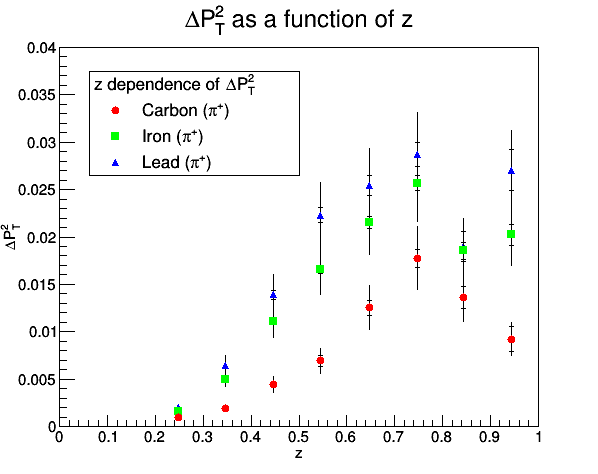
\includegraphics[width=7.4cm] {chap6-fig/F_PvZ.png} 
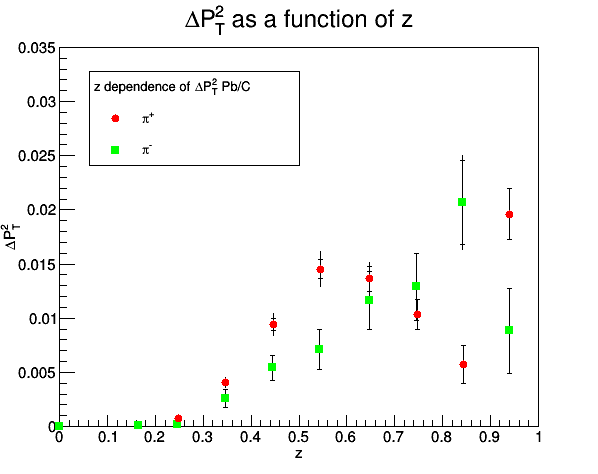
\includegraphics[width=7.4cm] {chap6-fig/F_PvZ_PbC.png} 
\caption {\dpt as a function of $z$. Left panel is the usual
observable, right panel shows multiplicity ratio of lead normalized to carbon. Normalization uncertainties are not shown.}
\label{fig:PZ}
\end{figure}

\subsubsection{$Q^2$ Dependence}

Finally, the $Q^2$ dependence of \dpt is an important result for the BDMPS based 
calculation from \cite{Domdey:2008aq}. They expect a raise of \dpt with $Q^2$,
which is not observed in the figure \ref{fig:PQ2}. Using
binning in $\nu$ and carbon based \dpt (figure \ref{fig:PQ2-detailed}) gives a similar
result. In conclusion, within error bars, no effect is observed for \dpt as a function of $Q^2$.
However, as theoretical input is missing, it is not clear if we have the resolution to observe
the effect expected within BDMPS based models.

\begin{figure}[tbp]
\centering
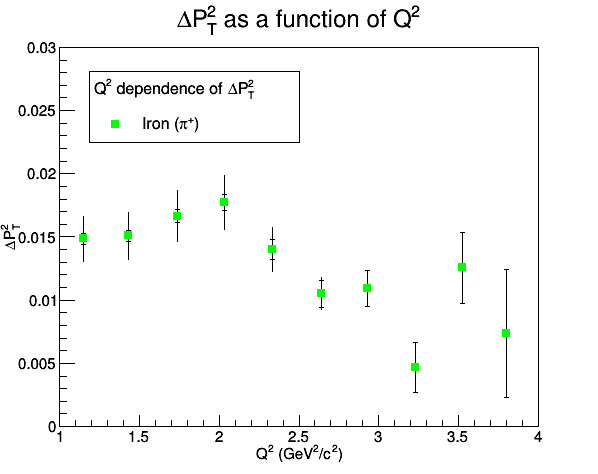
\includegraphics[width=7.4cm] {chap6-fig/F_PvQ2.png} 
\caption {\dpt for iron as a function of $Q^2$ (GeV$^2$/c$^2$) 
with usual cuts. Normalization uncertainties are not shown.}
\label{fig:PQ2}
\end{figure}

\begin{figure}[tbp]
\centering
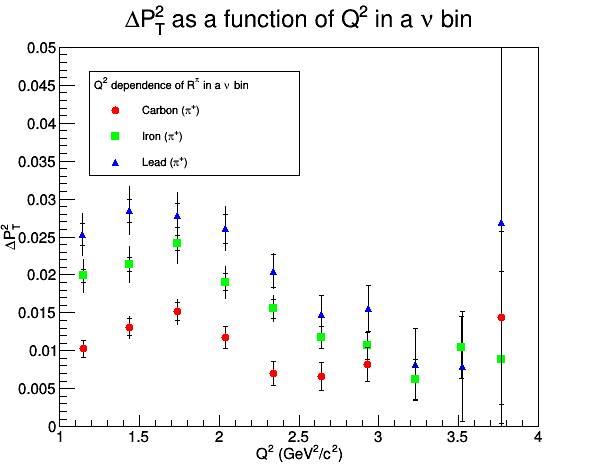
\includegraphics[width=7.4cm] {chap6-fig/F_PvQ2inNu.png} 
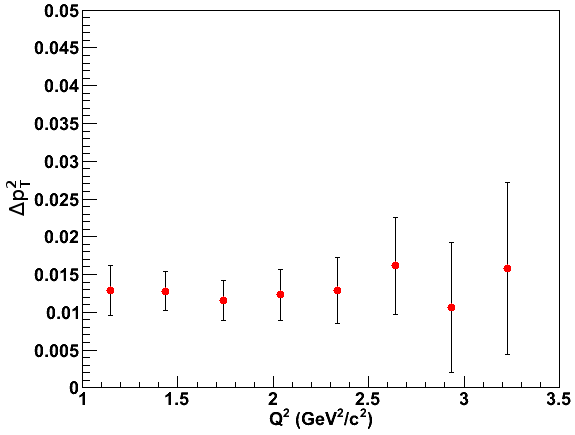
\includegraphics[width=7.4cm] {chap6-fig/F_PvQ2_PbC.png} 
\caption {\dpt as a function of $Q^2$ (GeV$^2$/c$^2$). Left panel is the usual
observable in a tight $\nu$ bin ($3.25 < \nu < 3.75$~GeV). Right panel shows \dpt 
of lead relative to carbon. Normalization uncertainties are not shown.}
\label{fig:PQ2-detailed}
\end{figure}

